\begin{subappendices}


%\renewcommand{\theequ}{\Alph{section}.\arabic{equ}}


\section{Calibration Solutions for the sky model tests }\label{ap:calib_solutions}
The output of the calibration step is a data set corrected for direction independent effects, as well as a set of calibration solutions. Figures \ref{fig:ch6_skymodel_rcalib_004_03} and \ref{fig:ch6_skymodel_rcalib_08_15} show the calibration solutions for core stations obtained when calibrating with sky models with minimum flux cutoffs of 0.05, 0.3, 0.8 and 1.5Jy. Much like in Figure \ref{fig:ch6_skymodel_images}, we can see that there is no significant difference between the calibration solutions for these stations. As a note, the naming scheme for LOFAR stations is CS/RS for core/remote stations, three digits for station number, HBA0/HBA1 for High Band antennas and LBA0/LBA1 for low-band antennas. The 0,1 suffixes correspond to sub-arrays in the core stations which can be correlated separately. Additionally, the CS/RS is replaced with the 2-letter country code for international stations\citep{staiton_data_cookbook}.

We compare the phase solutions for stations CS032HBA0 and CS003HBA0 and the reference station for two different calibrations in Figure \ref{fig:ch6_diffs_solutions}. We note that this difference is within 0.3 rad for the entire observation. Combined with the results in the other two plots, our results suggest that the calibration solutions do not degrade when calibration is done with a smaller sky model.

\begin{figure}
    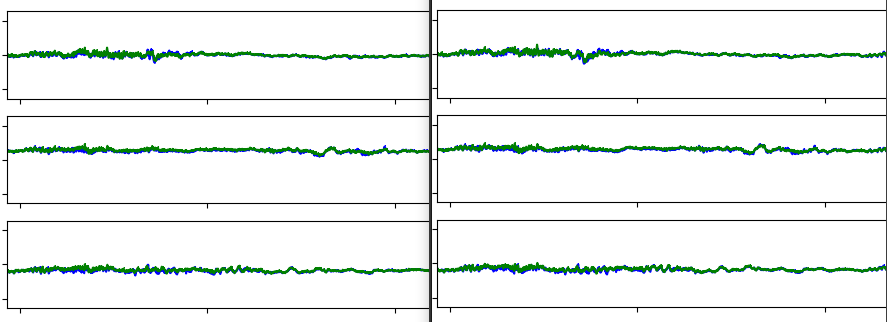
\includegraphics[width=0.95\linewidth]{ch6/figures/005_and_03_solutsions_CS003HBA0_CS003HBA1_CS004HBA0.png}
      \caption[Calibration Solutions for sky models with low flux cutoff]{The calibration (phase) solutions for the test data set obtained when calibrating with sky models of 0.05 Jy cutoff (left) and 0.3Jy cutoff (right). The data shows the phase solutions for baselines including stations CS003HBA0, CS003HBA1 and CS004HBA0, with respect to the reference station, CS001HBA0. The right solutions were obtained using the production calibration model. We do not see any improvement in results in the left figure, which took twice as long to obtain.}
	\label{fig:ch6_skymodel_rcalib_004_03}
\end{figure}

\begin{figure}
    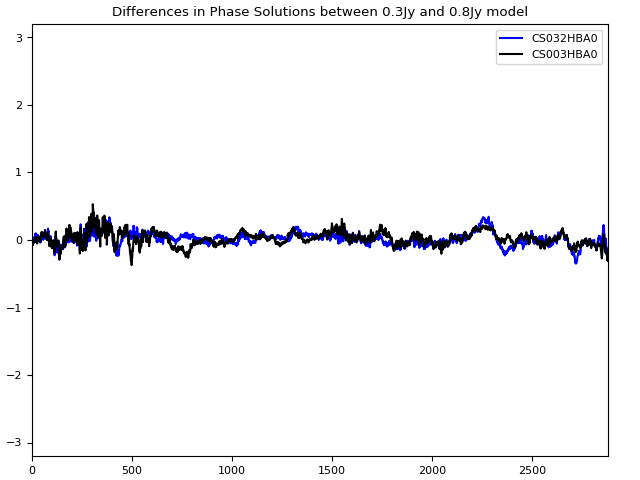
\includegraphics[width=0.9\linewidth]{ch6/figures/diffs.png}
      \caption[Calibration solution differences between two skymodels]{Difference of phase solutions between calibrations with the 0.3Jy and 0.8Jy sky models. The solutions for both stations are around zero phase for the duration of the observation.}
	\label{fig:ch6_diffs_solutions}
\end{figure}

\begin{figure}
    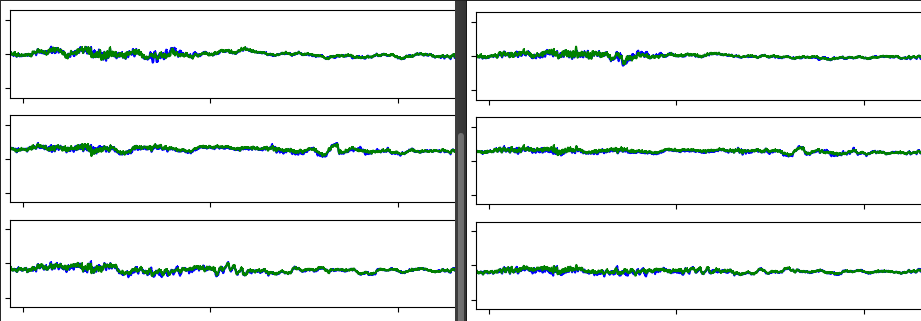
\includegraphics[width=0.95\linewidth]{ch6/figures/08_and_15_solutsions_CS003HBA0_CS003HBA1_CS004HBA0.png}
      \caption[Calibration solutions for sky models with high flux cutoff]{The calibration (phase) solutions for the test data set obtained when calibrating with sky models of 0.8 Jy cutoff (left) and 1.5Jy cutoff (right). The data shows the phase solutions for baselines including stations CS003HBA0, CS003HBA1 and CS004HBA0, with respect to the reference station, CS001HBA0. We can see that the calibration solutions shown here are not significantly different than those shown in \ref{fig:ch6_skymodel_rcalib_004_03}, despite taking a fraction of the processing time.  }
	\label{fig:ch6_skymodel_rcalib_08_15}
\end{figure}

\section{Parametric model parameters and fit accuracy}\label{ap:ch6_model_params}

In this section, we note the uncertainties to the models fit in Equations \ref{eq:ch6_runtime_size_models}-\ref{eq:ch6_download_model}. 

%Resetting the equation environment to match the equ number
\numberwithin{equation}{section}
\setcounter{equation}{6}
\renewcommand{\theequation}{\Alph{section}.\arabic{equation}}

\subsection{Fits quality of run time vs input size model}

The models of the processing time vs input size were fit as a linear regression. In this work we present such models for the {\fontfamily{qcr}\selectfont  gsmcal\_solve}, {\fontfamily{qcr}\selectfont gsmcal\_apply}, {\fontfamily{qcr}\selectfont dpppconcat}, {\fontfamily{qcr}\selectfont predict\_ateam} and {\fontfamily{qcr}\selectfont ateamcliptar}, the five slowest steps. The resulting models, calculated by the \texttt{scipy linregress}\citep{scipy} routine, are shown in Equation \ref{eq:ch6_runtime_size_models}. We present the $R^2$ values, P values and standard error below, in Table \ref{table:fits_size}.



\begin{table}[ht!]
\centering
\begin{tabular}{||p{2.2cm}| c | c|p{2cm}||} 
 \hline
 \texttt{prefactor} step & $R^2$ & P value & Standard Error \\ %[0.5ex]
 \hline
 predict\_ateam & 0.996   & 0                    & $1.92\times10^{-10}$    \\ 
 \hline
 ateamcliptar   & 0.979   & 0                    & $3.94\times10^{-11}$    \\ 
 \hline
 dpppconcat     & 0.999   & $1.2\times10^{-128}$ & $1.78\times10^{-10}$    \\ 
 \hline
 gsmcal\_solve $<=$16GB  & 0.995   & $3.12\times10^{-75}$ & $6.80\times10^{-9}$     \\ 
 \hline
 gsmcal\_solve $>$16GB  & 0.951   & $7.07\times10^{-40}$ & $1.58\times10^{-8}$     \\ 
 \hline
 gsmcal\_apply  & 0.989   & $5.6\times10^{-82}$  & $3.12\times10^{-10}$    \\ 

\hline
\end{tabular}
    \caption{Fit parameters for the models in Equation \ref{eq:ch6_runtime_size_models}. }
\label{table:fits_size}
\end{table}


\subsection{Fit of run time vs calibration model flux cutoff }

The run time vs Flux cutoff model shown in Equation \ref{eq:ch6_skymodel_flux} is defined by the equation $y=a\cdot x^{-k}$ and two parameters, $a$ and $k$. The covariance matrix for these two parameters is shown in Equation \ref{eq:cov_Flux}. The standard deviation for the fit of the parameters $a$ and $k$ is 26.134 and $7.624\times10^{-3}$ respectively.

\begin{equ}
\begin{equation}
  \begin{bmatrix}
    6.83\times10^{2}  &  -1.94\times10^{-1} \\
   -1.94\times10^{-1} &   5.81\times10^{-5} \\
\end{bmatrix}
\end{equation}
\caption{The covariance matrix of the parameters in model in Equation \ref{eq:ch6_skymodel_flux}.}
\label{eq:cov_Flux}
\end{equ}

\subsection{Fit of the NCPU model }
The covariance matrix for the fit parameters of equation \ref{eq:ch6_gsmcal_NCPU}, $a$ and $k$ in $y=a+\frac{k}{\mathcal{N}}$ are shown in Equation \ref{eq:cov_NCPU}. The standard deviation of the fits for $a$ and $k$ are 13.11 and 48.20 respectively. 

\begin{equ}
\begin{equation}
  \begin{bmatrix}
    171.94 & -504.11 \\
    -504.11 & 2322.95
\end{bmatrix}
\end{equation}
    \caption[Covariance matrix for parameters predicting run time from NCPU]{The covariance matrix for the parameters for the model predicting run time vs Number of CPUs used, shown in Equation \ref{eq:ch6_gsmcal_NCPU}.}
\label{eq:cov_NCPU}
\end{equ}

\subsection{Fit for the queuing time model}

The statistics of the model fit parameters for the queuing time model (Equation \ref{eq:ch6_queue_model}) are in Table \ref{table:fits_queue}. 
The queuing model is fit to the $75^{th}$ percentile of the queuing times for each parameter step. Since this results in a single number for each step, the model's P values are larger than the models from the other sections. 

\begin{table}[ht!]
\centering
\begin{tabular}{||p{2.2cm}| c | c|p{2cm}||} 
 \hline
 Value of $\mathcal{N}$ & $R^2$ & P value & Standard Error \\ %[0.5ex]
 \hline
 $\mathcal{N}\leq4$ & 0.382   & 0.381                   & 37.086    \\ 
 $\mathcal{N}>4$    & 0.986   & 0.075                   & 86.293    \\ 
\hline
\end{tabular}
    \caption[Goodness of fit parameters for the model in Equation \ref{eq:ch6_queue_model}.]{Goodness of fit parameters for the model in Equation \ref{eq:ch6_queue_model}. Since the model is split into two parts, we treat each section as a single linear model.}
\label{table:fits_queue}
\end{table}


\subsection{Fit of the download and extract model }
Equation \ref{eq:cov_downl} shows the covariance matrix for the two parameters  $a$ and $k$, $y=a\times10^{k}$ with the best fit values shown in Equation \ref{eq:ch6_download_model}. The standard deviations of the fits for $a$ and $k$ are 0.016 and 0.068 respectively. 

\begin{equ}
\begin{equation}
  \begin{bmatrix}
    2.53\times10^{-4} & 1.08\times10^{-3} \\
    1.08\times10^{-3} & 4.60\times10^{-3}
\end{bmatrix}
\end{equation}
\caption{The covariance matrix for the parameters for the model for Download and Extract time, shown in Equation \ref{eq:ch6_download_model}.}
\label{eq:cov_downl}
\end{equ}

\end{subappendices}
